\documentclass[tikz,border=5pt]{standalone}
\usepackage{tikz}
\usetikzlibrary{arrows.meta,positioning}
\definecolor{nebula}{HTML}{6366F1}
\definecolor{spark}{HTML}{14B8A6}
\definecolor{ink}{HTML}{334155}
\begin{document}
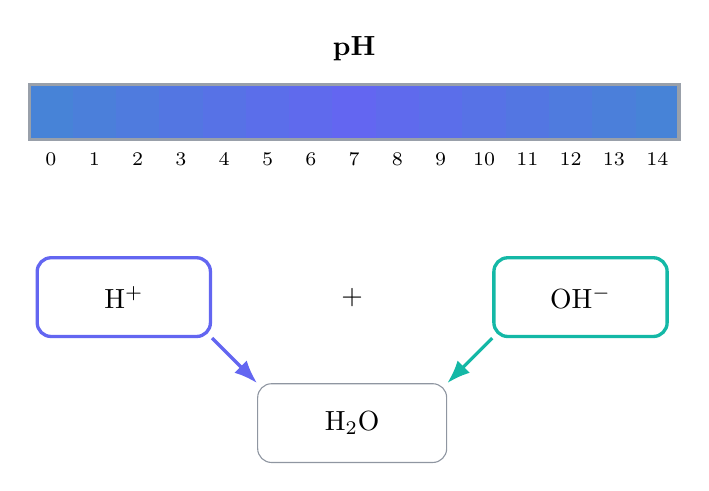
\begin{tikzpicture}[font=\sffamily,>=Latex]
  \foreach \x in {0,...,14} {
    \pgfmathsetmacro{\tone}{100-5*abs(\x-7)}
    \fill[nebula!\tone!spark] (\x*.55,0) rectangle ++(.55,.7);
    \node[font=\scriptsize] at (\x*.55+.275,-.25) {\x};
  }
  \draw[very thick,ink!50] (0,0) rectangle (8.25,.7);
  \node[font=\bfseries] at (4.125,1.15) {pH};
  \node[draw=nebula,very thick,rounded corners=5pt,minimum width=2.2cm,minimum height=1cm] (a) at (1.2,-2) {$\mathrm{H^+}$};
  \node[draw=spark,very thick,rounded corners=5pt,minimum width=2.2cm,minimum height=1cm] (b) at (7.0,-2) {$\mathrm{OH^-}$};
  \node[draw=ink!55,rounded corners=5pt,minimum width=2.4cm,minimum height=1cm] (w) at (4.1,-3.6) {$\mathrm{H_2O}$};
  \draw[->,very thick,nebula] (a.south east)--(w.north west);
  \draw[->,very thick,spark] (b.south west)--(w.north east);
  \node[fill=white,inner sep=3pt] at (4.1,-2) {$+$};
\end{tikzpicture}
\end{document}
